\documentclass[]{beamer} 
\setbeamerfont{all}{size=\large}
\setbeamerfont*{itemize/enumerate body}{size=\large}
\setbeamerfont*{itemize/enumerate subbody}{parent=itemize/enumerate body}
\setbeamerfont*{itemize/enumerate subsubbody}{parent=itemize/enumerate body}
\beamertemplatenavigationsymbolsempty
\usetheme{default}
\useinnertheme{circles}
\usebeamerfont{all}
\DeclareMathOperator*{\argmin}{arg\,min}
\usepackage{listings}
\usepackage{amssymb}
\usepackage{docmute}
\usepackage{hyperref}
\begin{document}

%\hspace*{\fill} \\

\title{Faster Image Segmentation with ENet}
\author{Nicholas Dronen}

\begin{frame}
\maketitle
\end{frame}

%\input{01-inception}
%\input{02-enet}
%\input{03-distillation}

\begin{frame}{Image Segmentation}
\centering
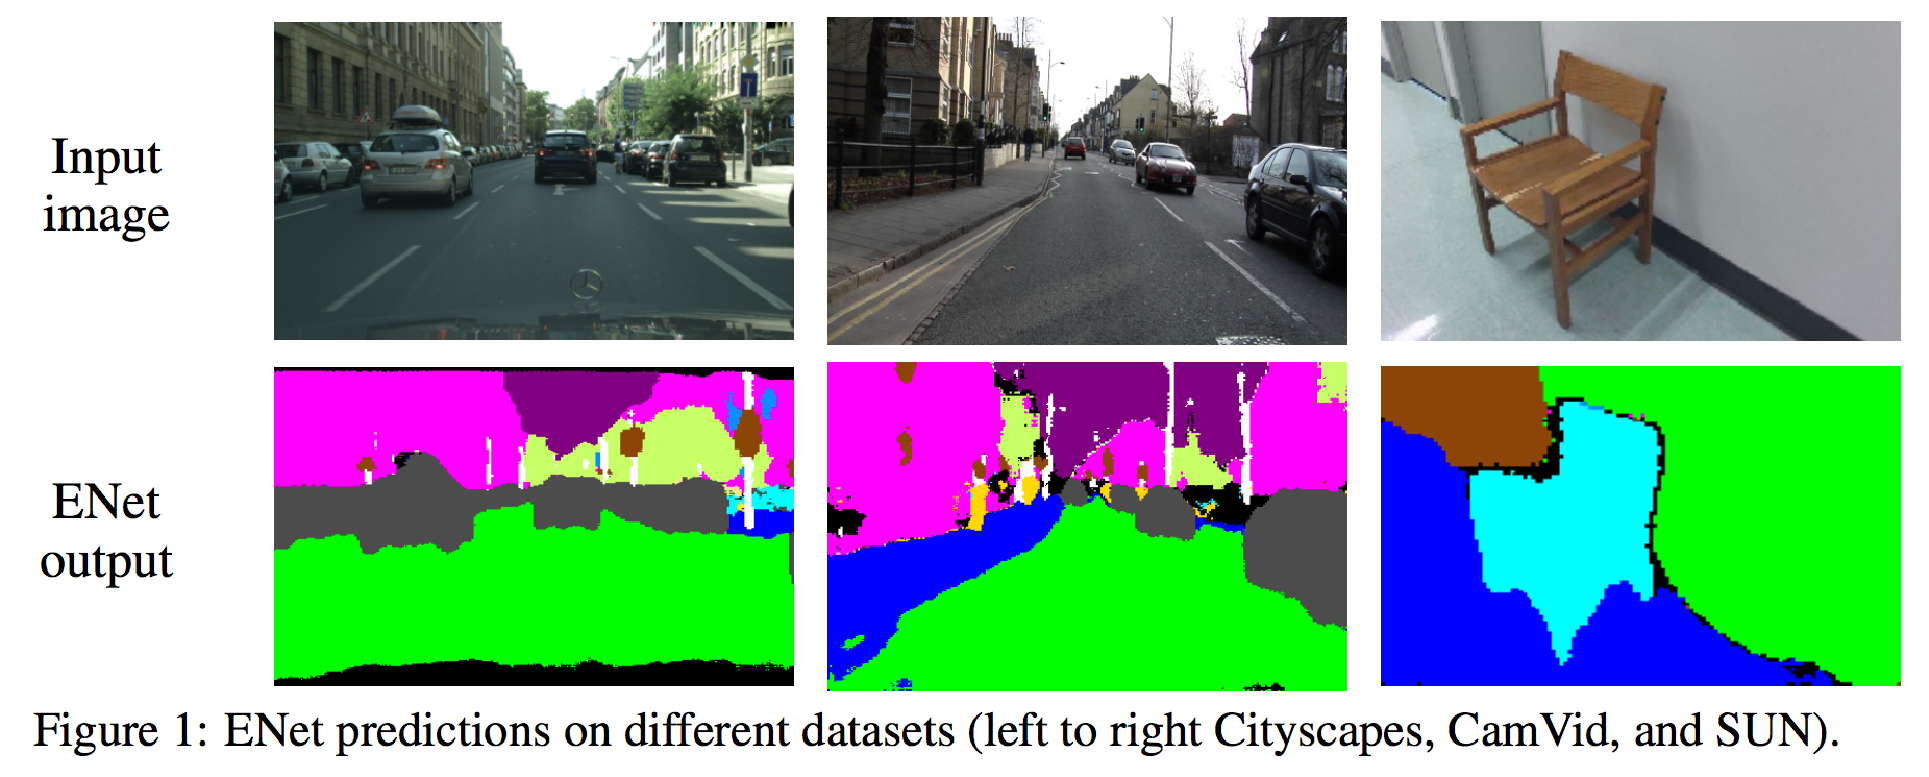
\includegraphics[width=0.95\textwidth]{figures/segmentation} \\
\end{frame}

\begin{frame}
\centering
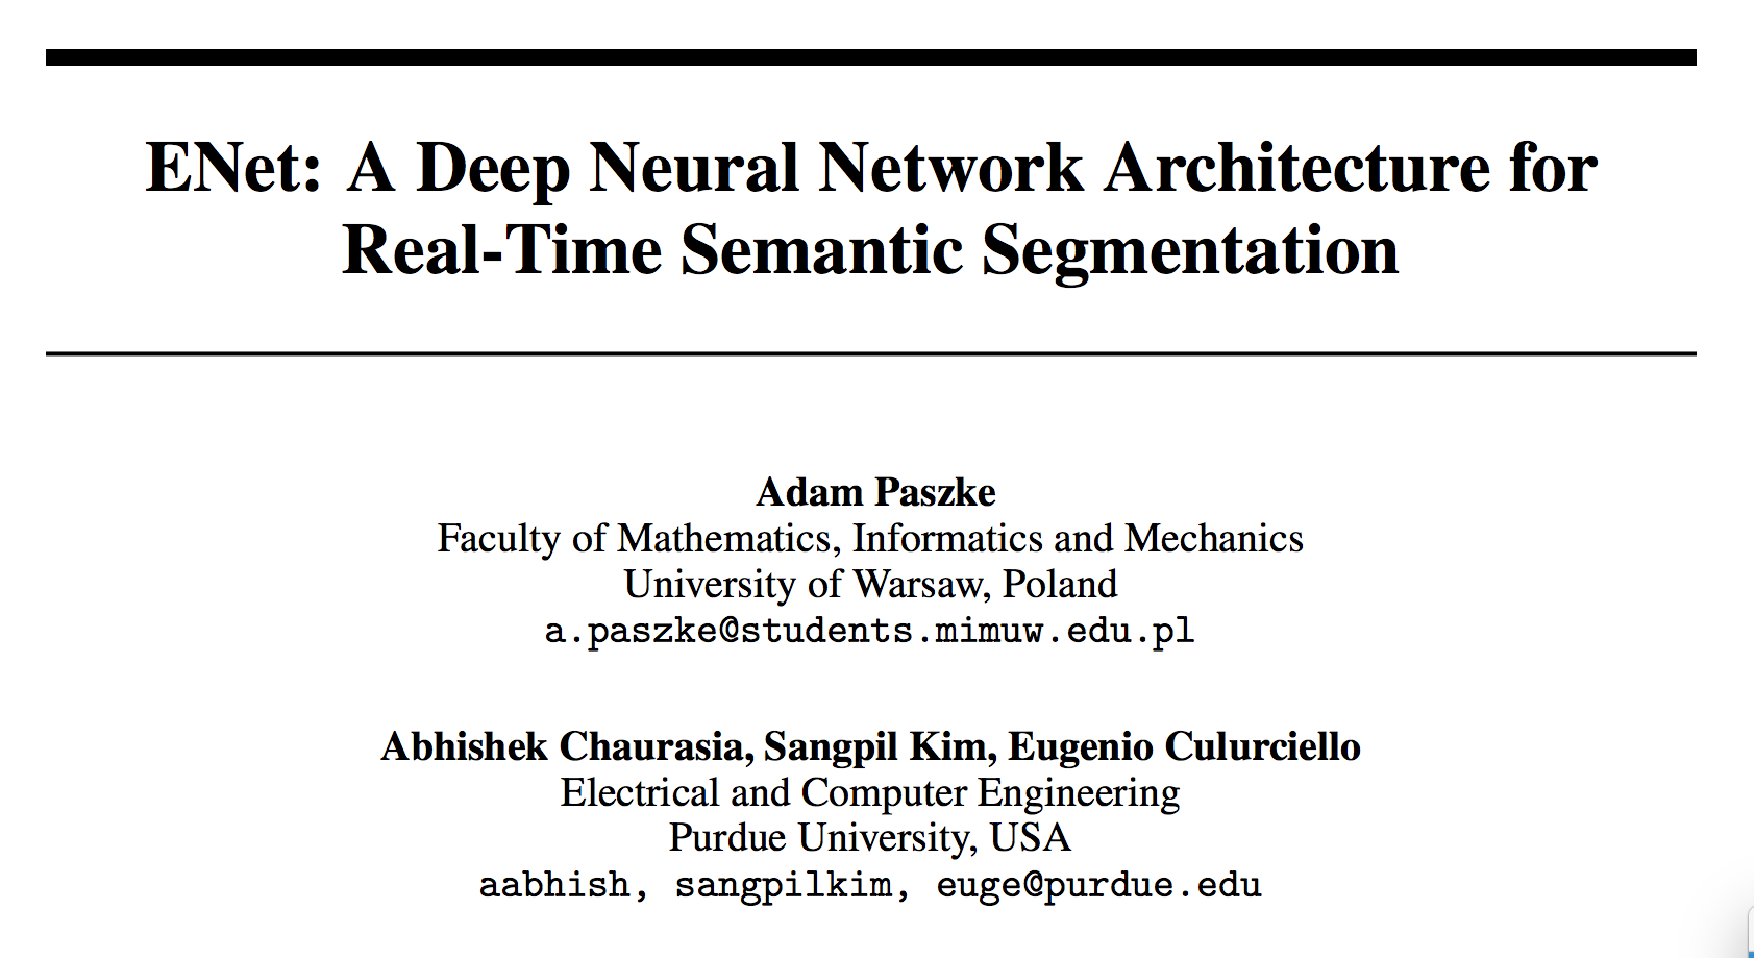
\includegraphics[width=0.9\textwidth]{figures/enet-title} \\
\href{https://arxiv.org/abs/1606.02147}{\textcolor{blue}{arXiv:0706.1234v1 [cs.CV]}}
\end{frame}

\begin{frame}{ENet versus SegNet: Inference Speed}
\centering
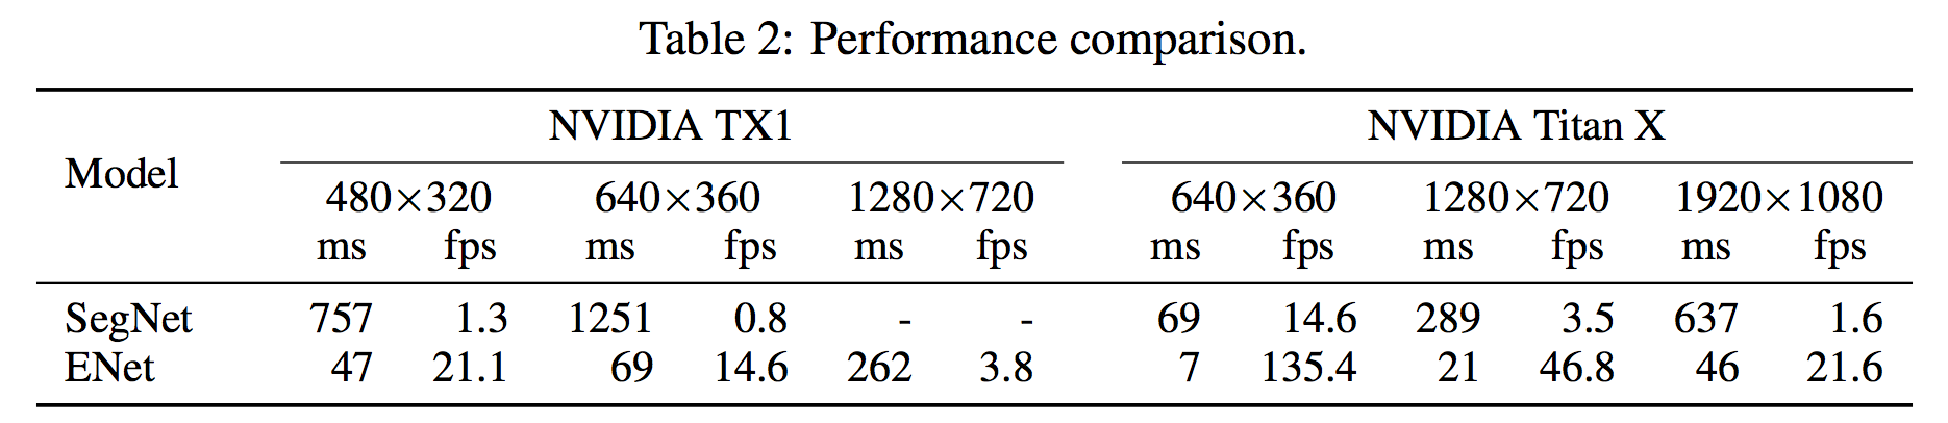
\includegraphics[width=0.9\textwidth]{figures/enet-vs-segnet-speed} \\
\hspace*{\fill} \\
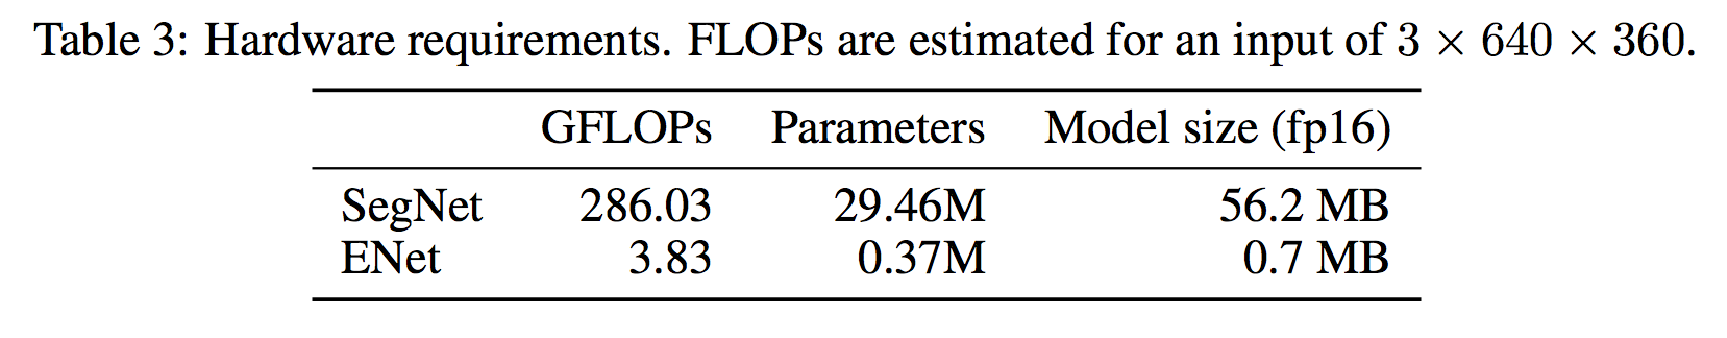
\includegraphics[width=0.9\textwidth]{figures/enet-vs-segnet-gflops-size}
\end{frame}

\begin{frame}{ENet versus SegNet: Benchmark Data}
\begin{itemize}
\item Cityscapes: road, 2975 train/1525 test, 19 classes
\item CamVid: road, 367 train/233 test, 11 classes
\item SUN RGB-D: interior, 5285 train/5050 test, 37 classes
\end{itemize}
\end{frame}

\begin{frame}{ENet Cityscapes segmentations}
\centering
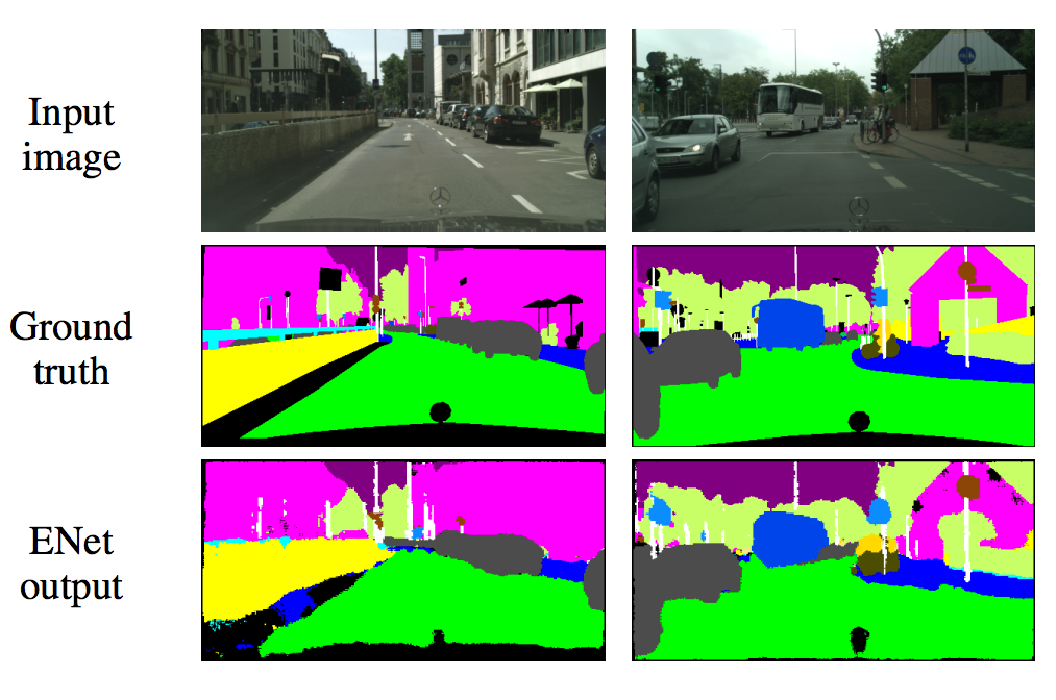
\includegraphics[width=0.9\textwidth]{figures/enet-cityscapes}
\end{frame}

\begin{frame}{ENet CamVid segmentations}
\centering
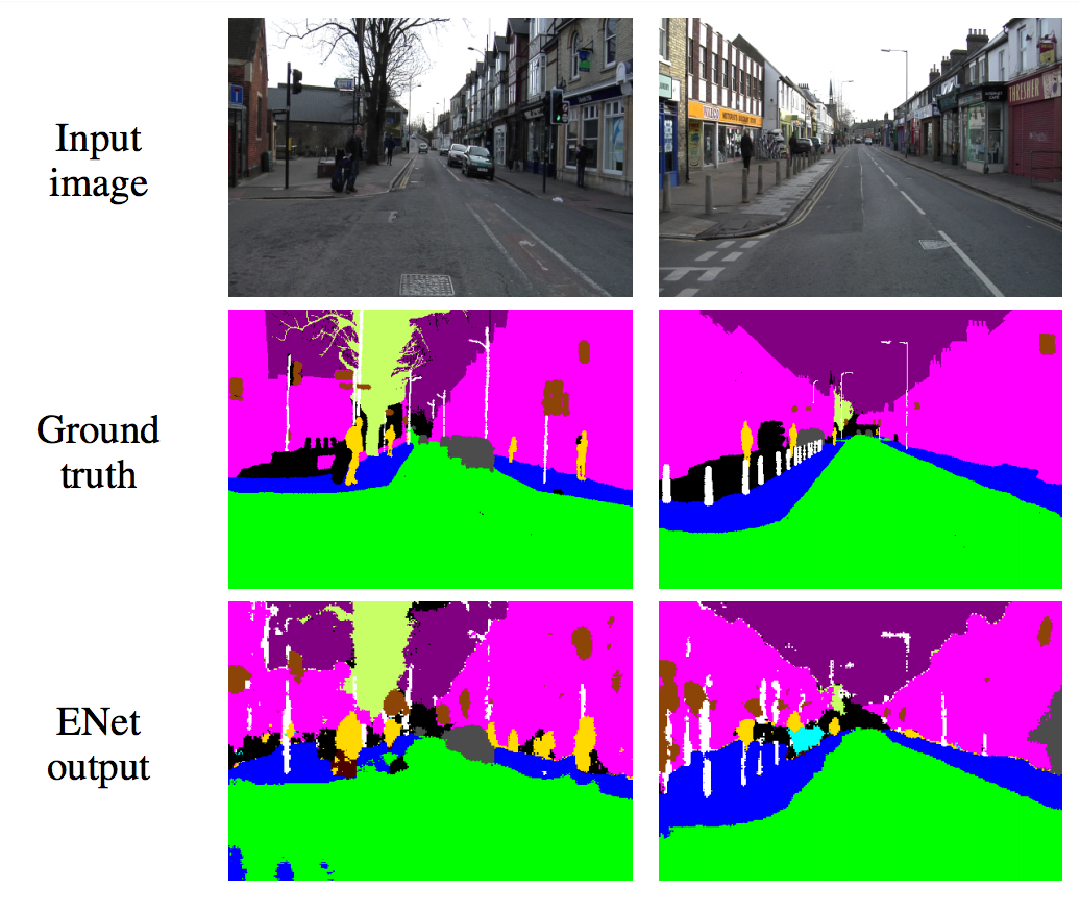
\includegraphics[width=0.9\textwidth]{figures/enet-camvid}
\end{frame}

\begin{frame}{ENet SUN RGB-D segmentations}
\centering
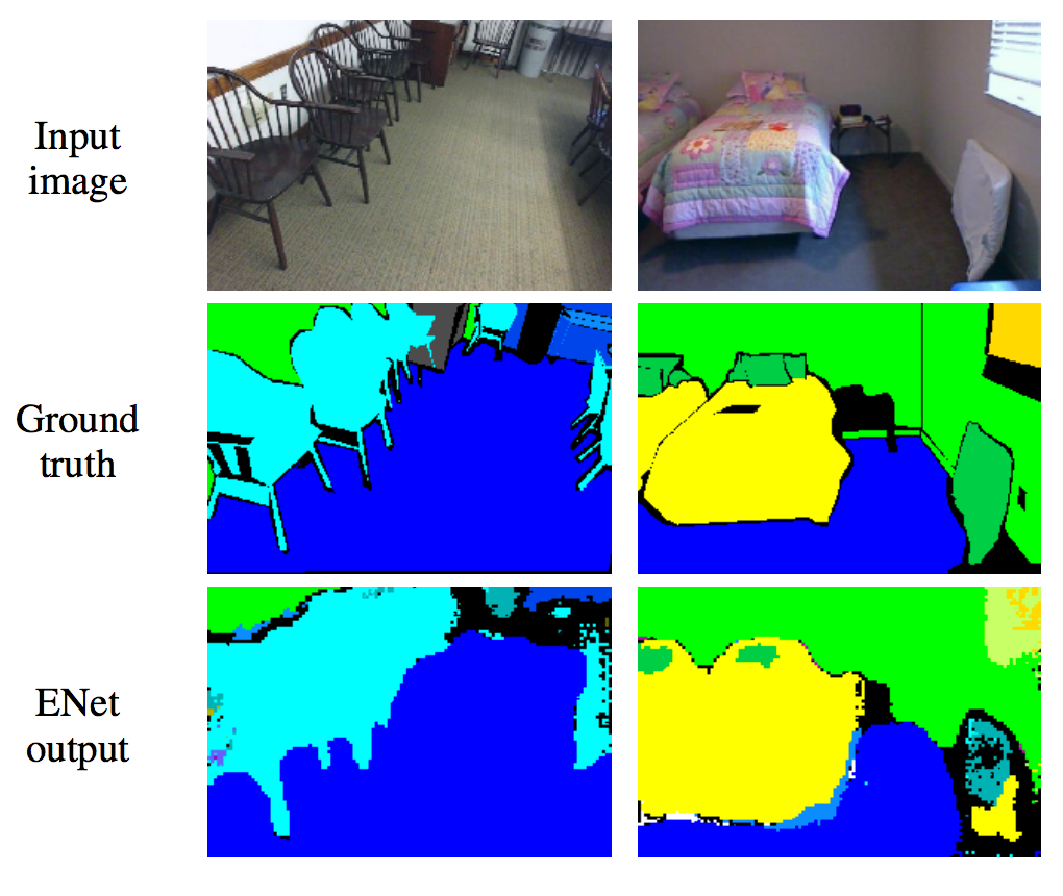
\includegraphics[width=0.9\textwidth]{figures/enet-sun-rgbd}
\end{frame}

\begin{frame}{ENet versus SegNet: Model Accuracy}
\centering
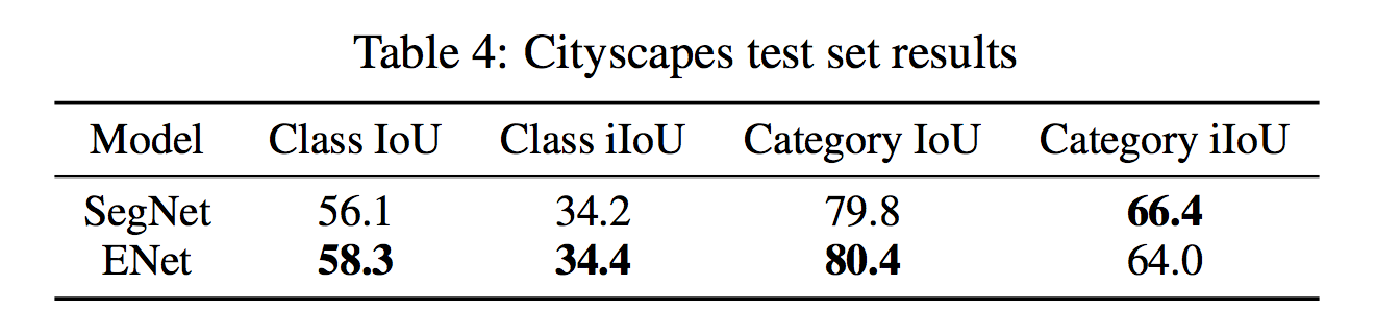
\includegraphics[scale=0.325]{figures/enet-versus-segnet-accuracy-1-cityscapes} \\
\hspace*{\fill} \\
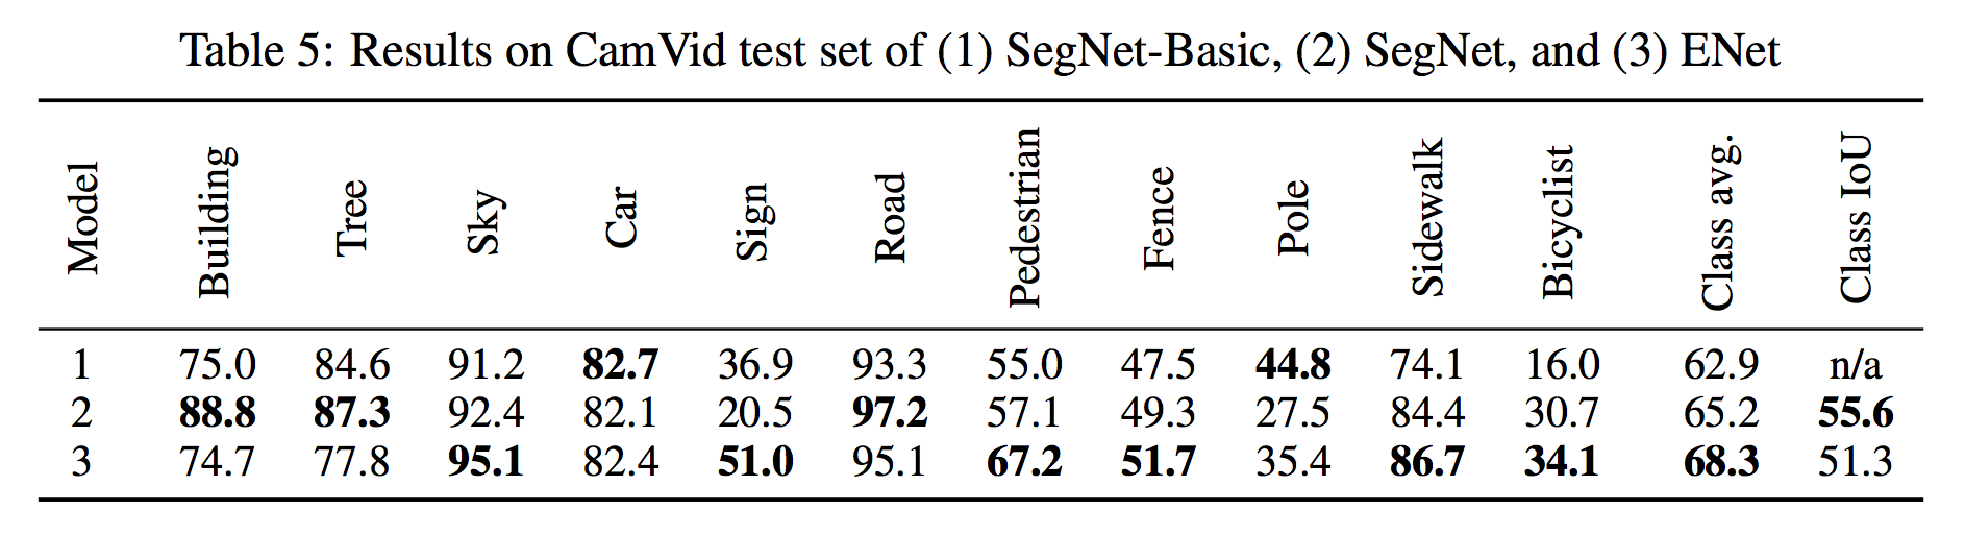
\includegraphics[scale=0.325]{figures/enet-versus-segnet-accuracy-2-camvid} \\
\hspace*{\fill} \\
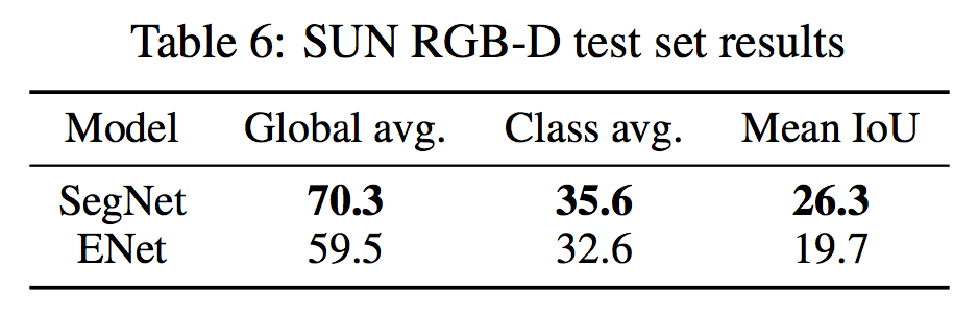
\includegraphics[scale=0.325]{figures/enet-versus-segnet-accuracy-3-sun-rgbd} \\
\end{frame}

\begin{frame}{Prior work: FCN}
\centering
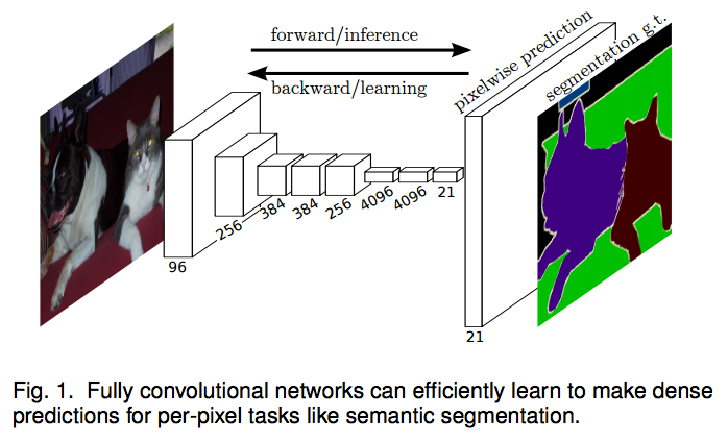
\includegraphics[width=0.95\textwidth]{figures/fcn-1} \\
\href{https://arxiv.org/abs/1605.06211}{\textcolor{blue}{Fully Convolutional Networks for Semantic Segmentation, Shelhamer et al, arXiv:1605.06211 [cs.CV]}}
\end{frame}

\begin{frame}{Prior work: FCN}
\centering
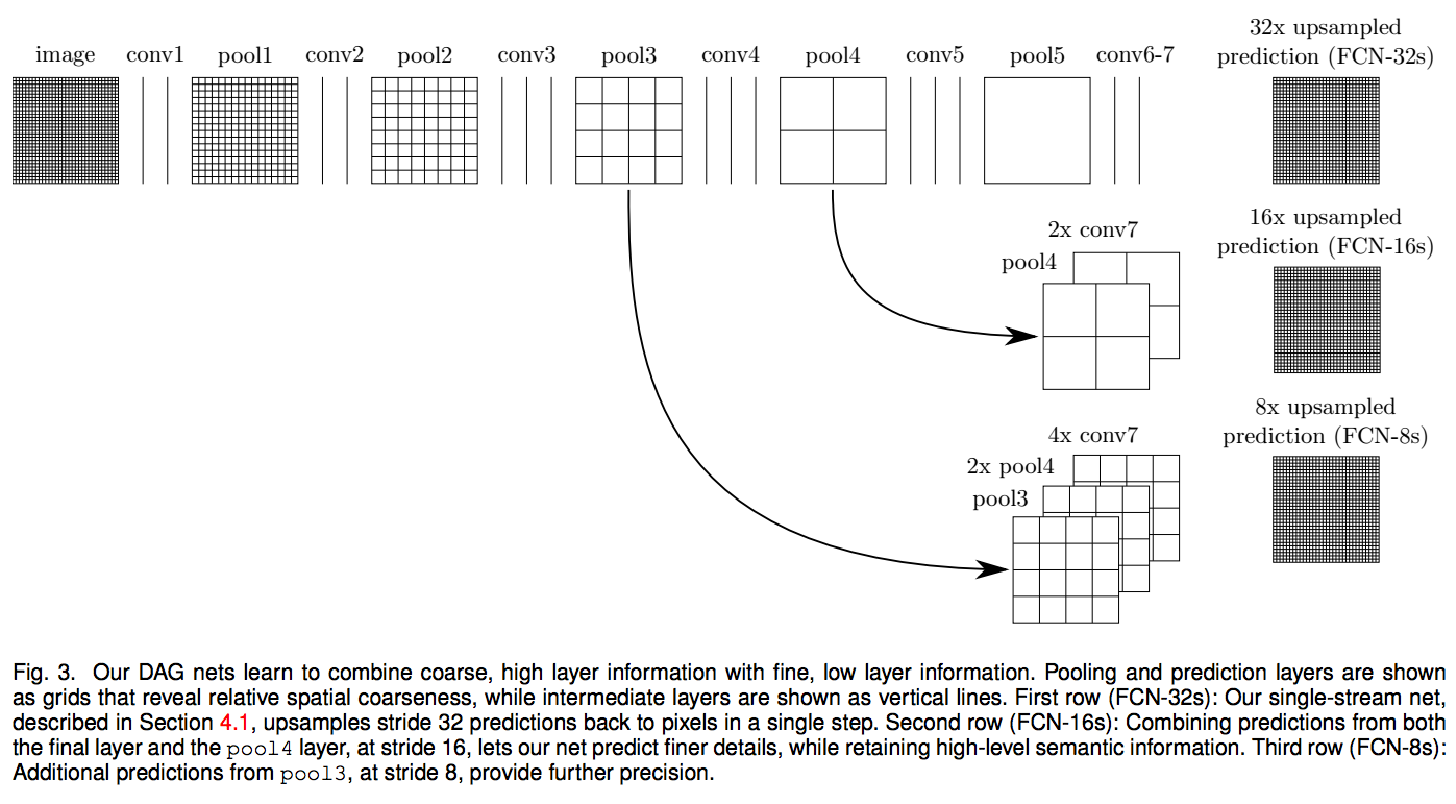
\includegraphics[width=0.95\textwidth]{figures/fcn-2} \\
\href{https://arxiv.org/abs/1605.06211}{\textcolor{blue}{Fully Convolutional Networks for Semantic Segmentation, Shelhamer et al, arXiv:1605.06211 [cs.CV]}}
\end{frame}

\begin{frame}{Prior work: FCN}
\centering
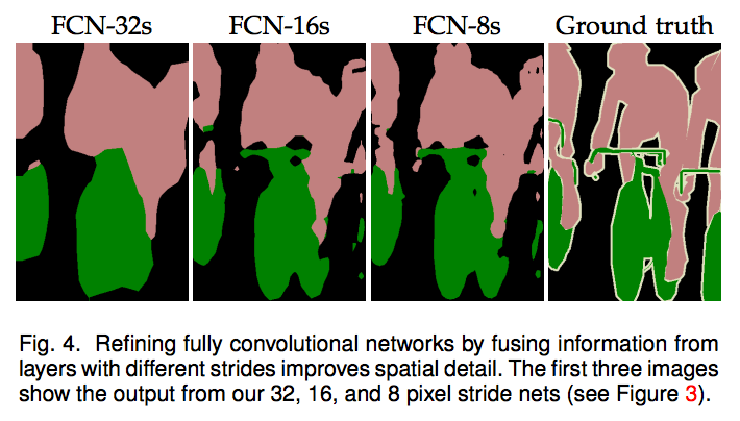
\includegraphics[width=0.95\textwidth]{figures/fcn-3} \\
\href{https://arxiv.org/abs/1605.06211}{\textcolor{blue}{Fully Convolutional Networks for Semantic Segmentation, Shelhamer et al, arXiv:1605.06211 [cs.CV]}}
\end{frame}

\begin{frame}{Prior work: SegNet}
\centering
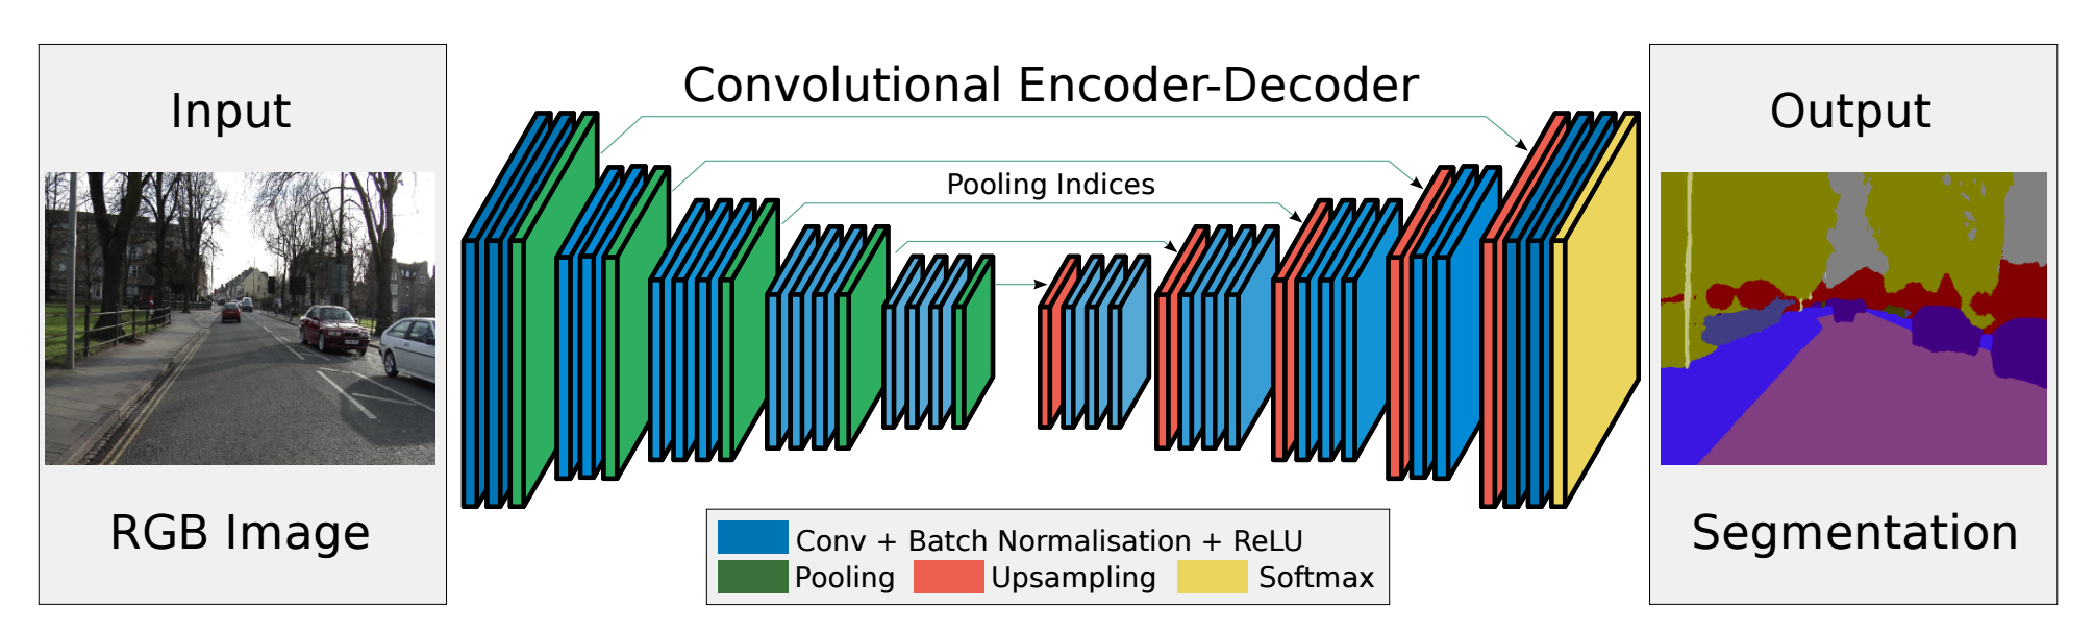
\includegraphics[width=0.95\textwidth]{figures/segnet} \\
\href{https://arxiv.org/abs/1511.00561}{\textcolor{blue}{
SegNet: A Deep Convolutional Encoder-Decoder Architecture for Image Segmentation, Badrinarayanan et al, arXiv:1511.00561v3 [cs.CV]}}
\end{frame}


\begin{frame}{ENet Architecture}
\centering
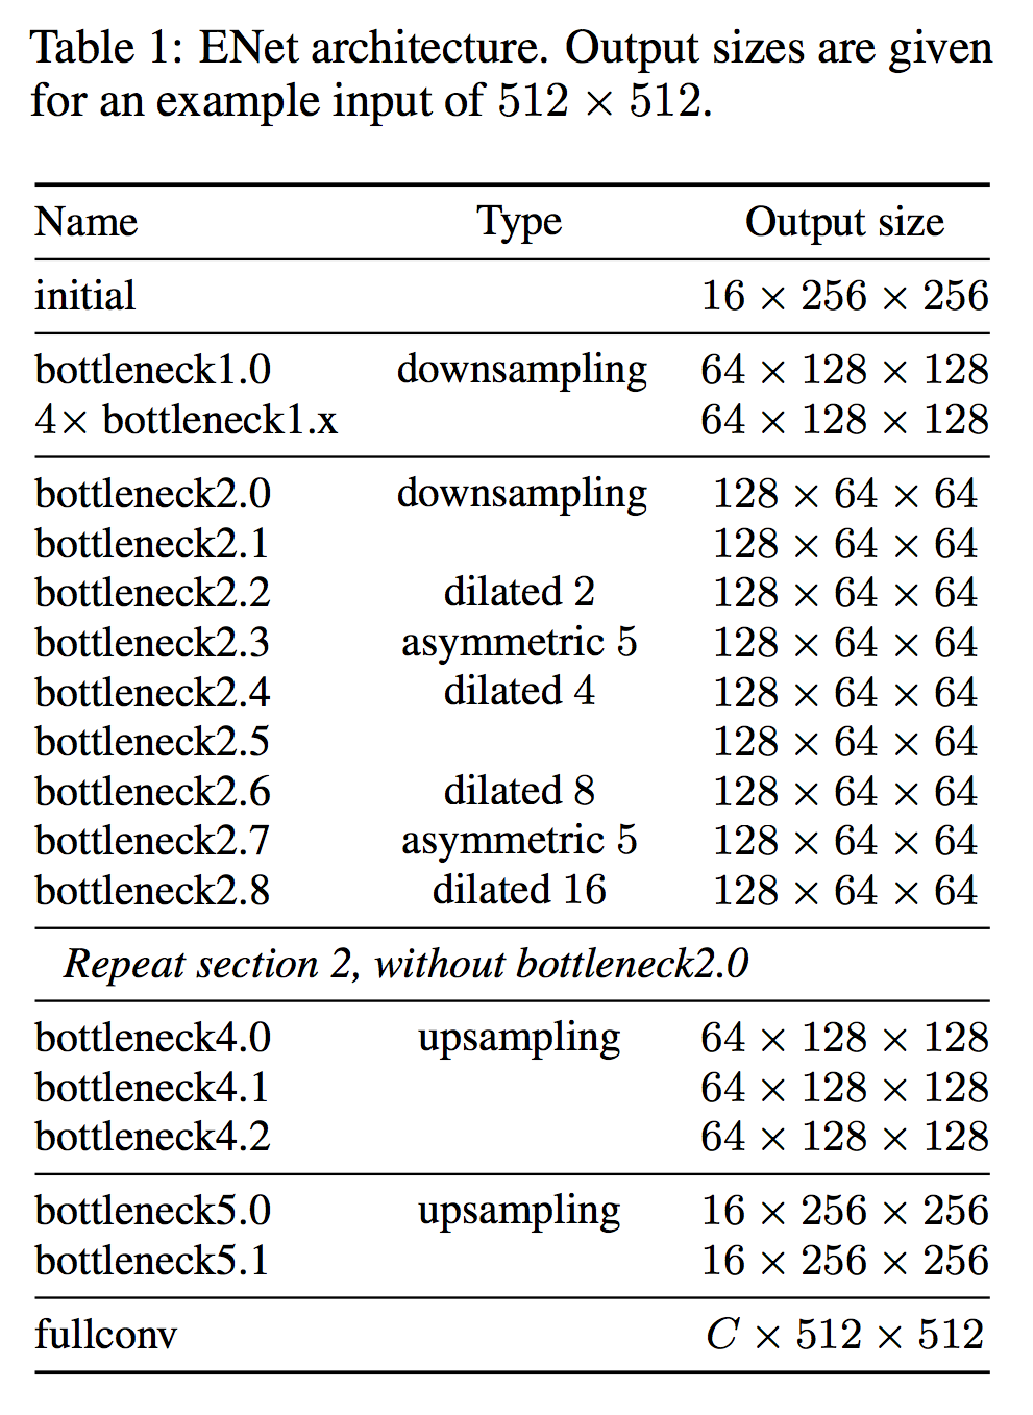
\includegraphics[height=0.9\textheight]{figures/enet-architecture}
\end{frame}

\begin{frame}{ENet Layers}
\centering
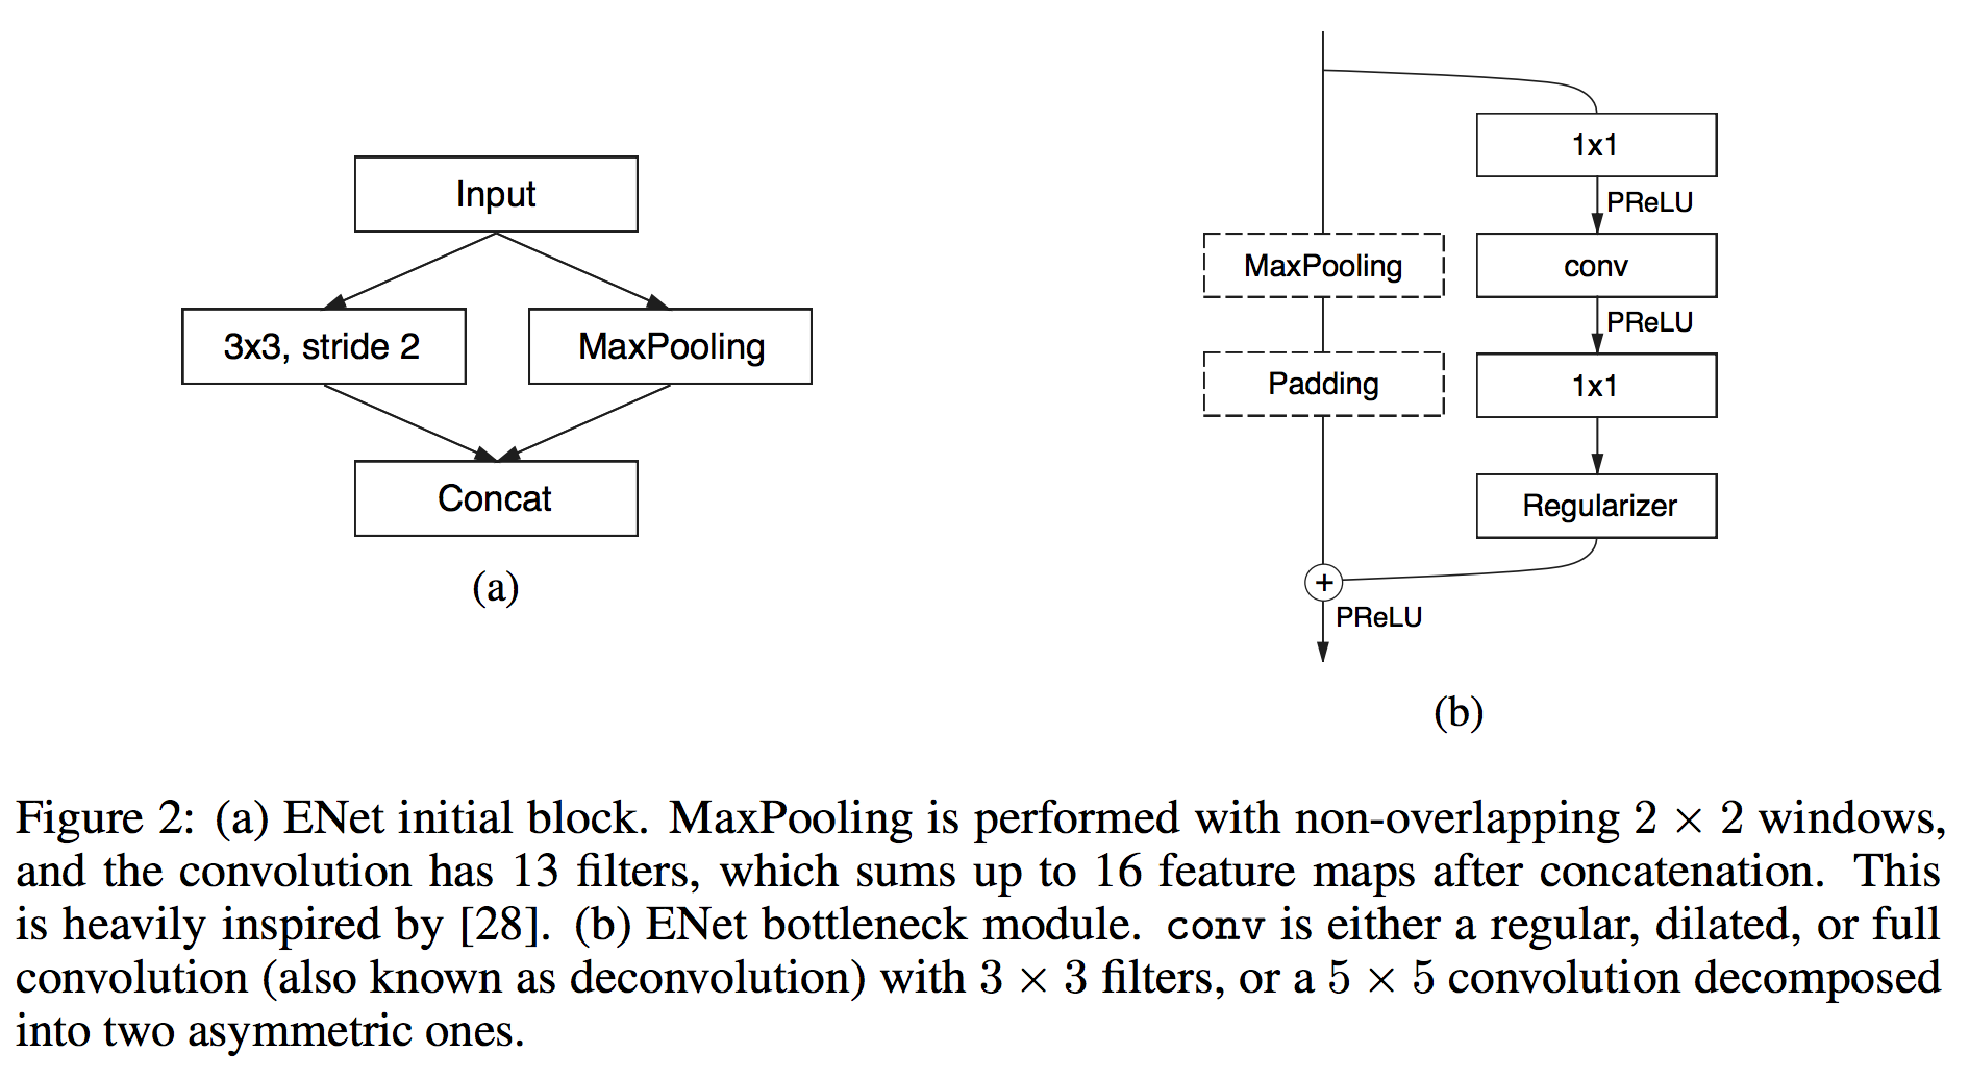
\includegraphics[scale=0.325]{figures/enet-layers}
\end{frame}

\begin{frame}{ENet Tricks}
\begin{itemize}
\item Speed 
  \begin{itemize}
  \item Early downsampling.
  \item Minimize cuDNN kernel calls (no bias).
  \item $1 \times 1$ convolutions (dim. reduction along \emph{filters}).
  \item Asymmetric convolutions: $3 \times 3 \to 1 \times 3, 3 \times 1$
  \end{itemize}
\item Accuracy
  \begin{itemize}
  \item Dilated convolutions.
  \item No batch normalization, etc.
  %\item 16-block encoder; 5-block, 1-layer decoder.
  \end{itemize}
\end{itemize}
\end{frame}

\begin{frame}{$1 \times 1$ Convolutions}
\centering
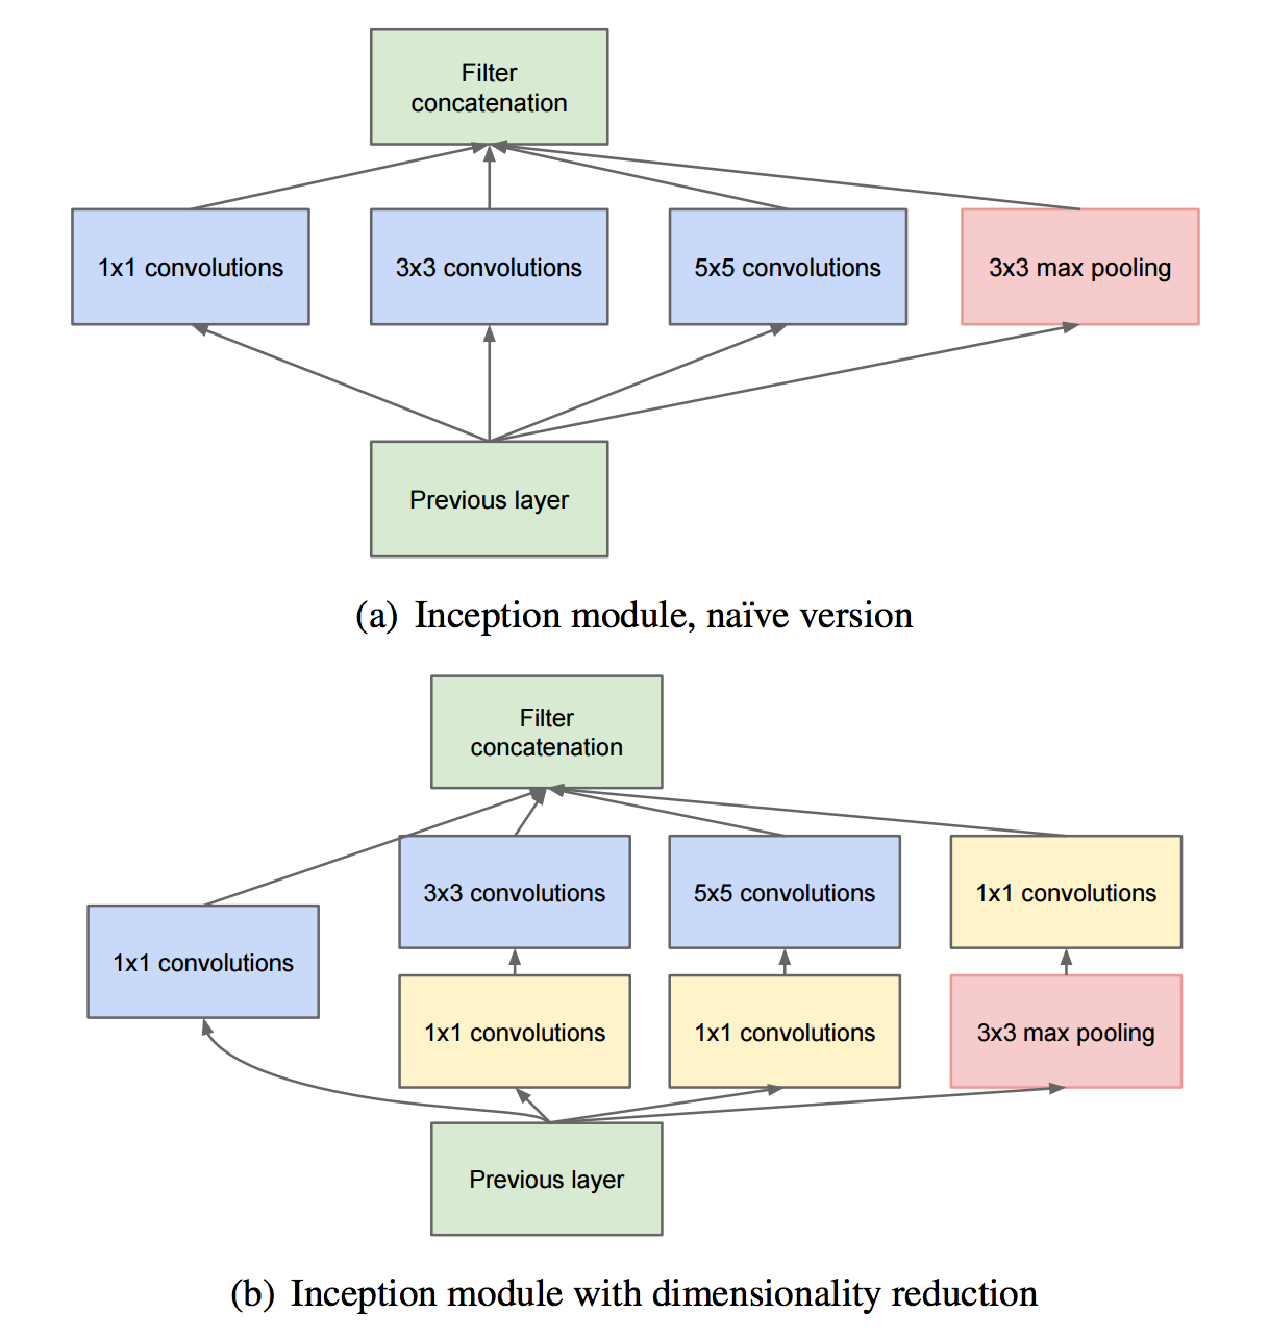
\includegraphics[scale=0.375]{figures/1x1-convolutions}
\end{frame}

\begin{frame}{Asymmetric Convolutions}
\centering
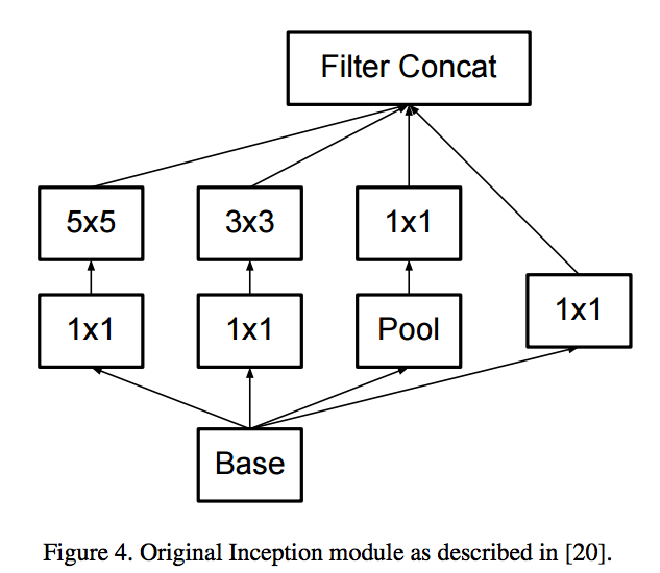
\includegraphics[scale=0.375]{figures/inception-assymetric-1}
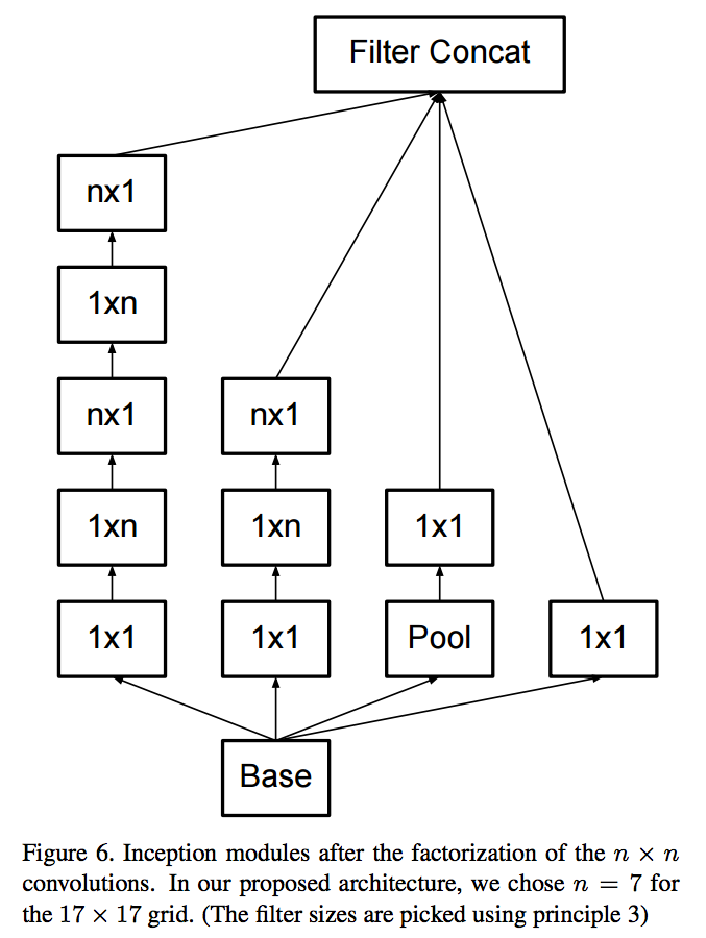
\includegraphics[scale=0.375]{figures/inception-assymetric-2}
\end{frame}

%\begin{frame}{TODO: add figure for assymetric convolutions}
%\centering
%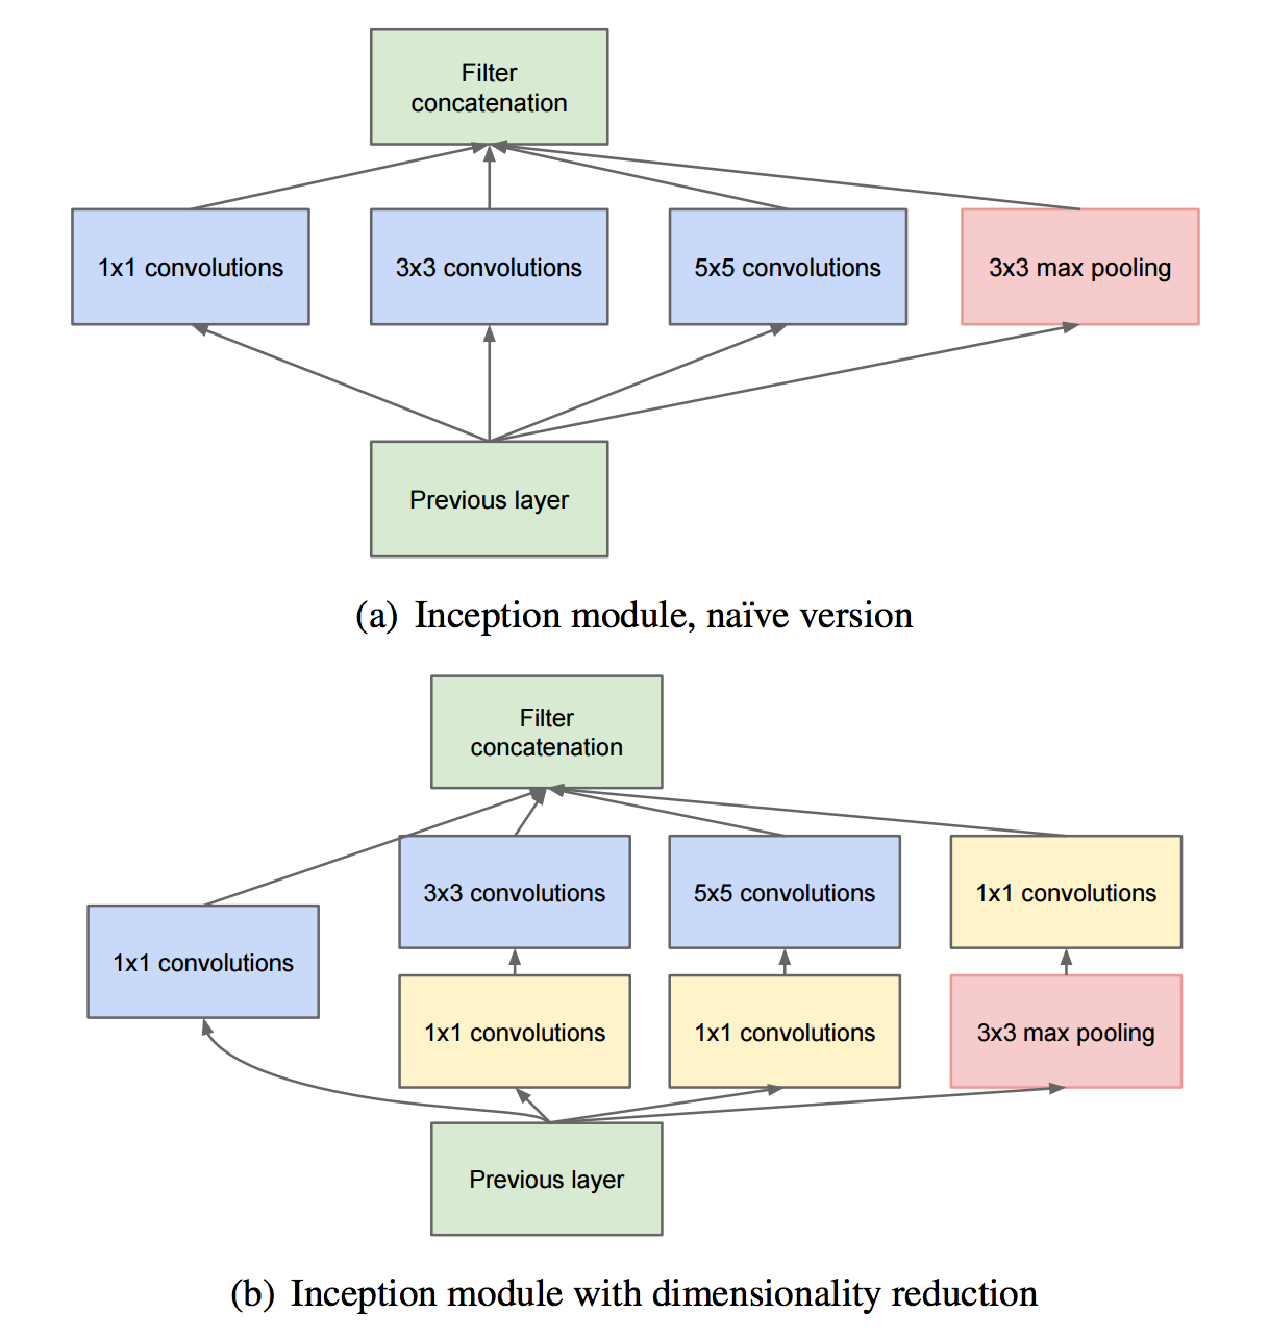
\includegraphics[scale=0.375]{figures/1x1-convolutions}
%\end{frame}

\begin{frame}{Dilated Convolutions}
\centering
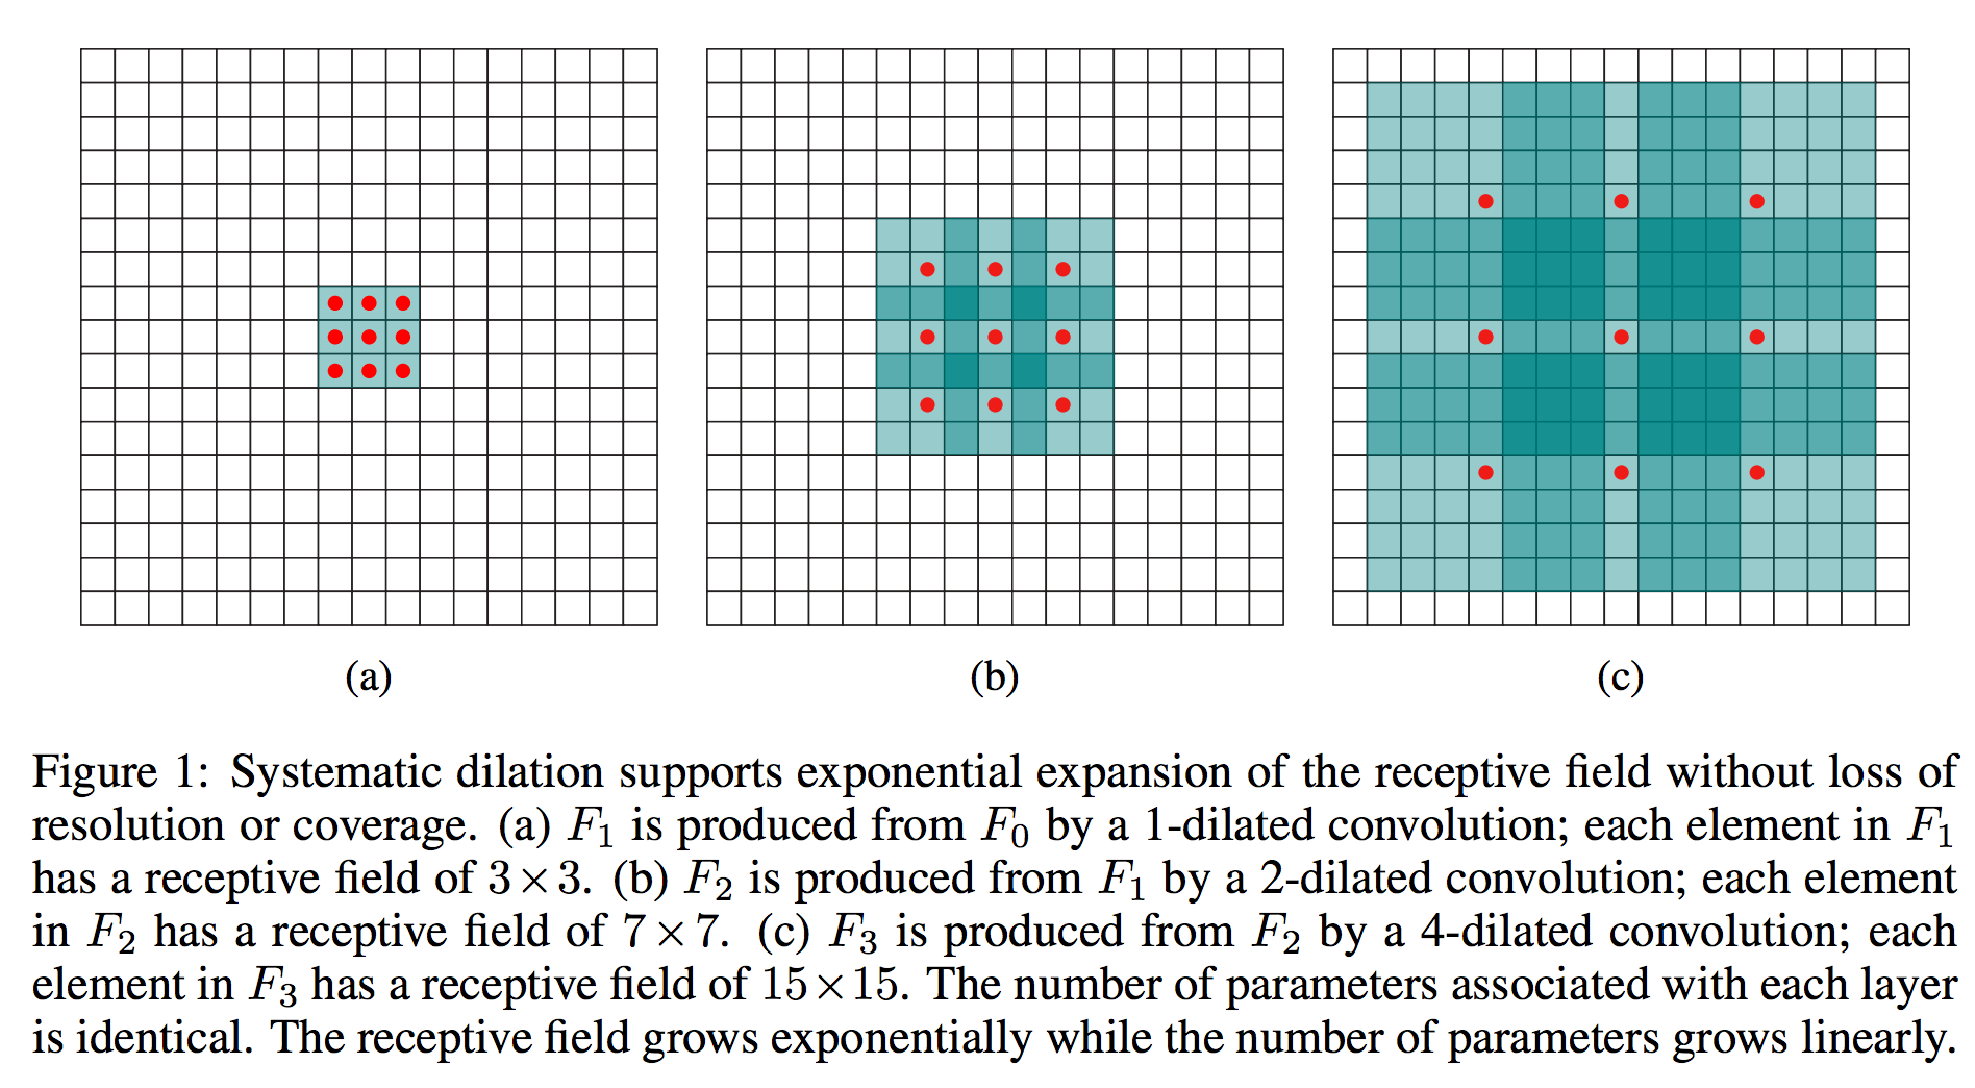
\includegraphics[scale=0.325]{figures/dilated-convolutions}
\end{frame}

\begin{frame}{PReLU and the identity function}
\centering
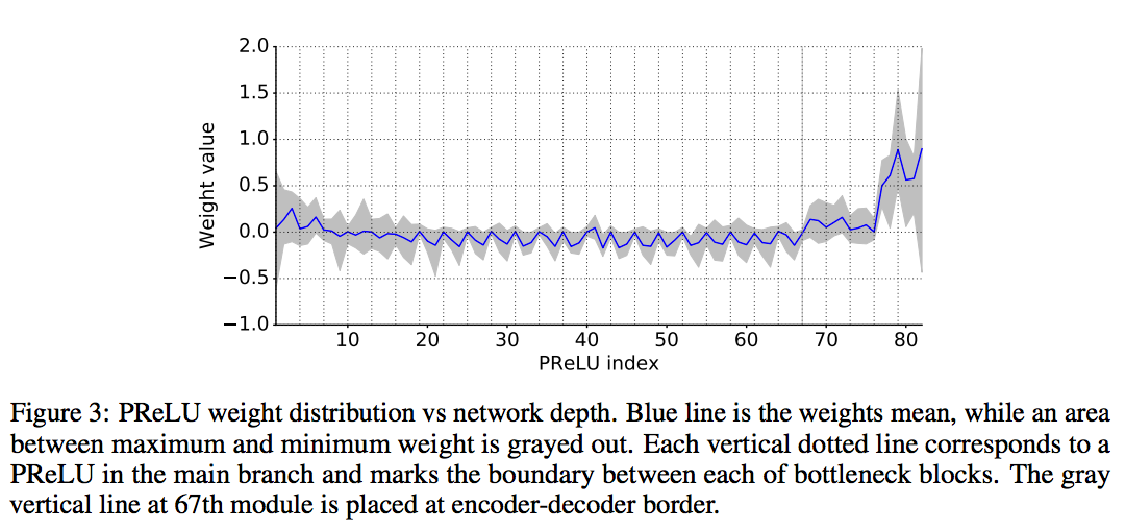
\includegraphics[width=0.95\textwidth]{figures/enet-prelu}
\end{frame}

%\begin{frame}{Dilated Convolutions}
%\begin{itemize}
%\item \href{https://github.com/BVLC/caffe/pull/3452/files}{\textcolor{blue}{Caffe pull request\#3452}}
%\item \href{http://arxiv.org/abs/1509.03371}{\textcolor{blue}{Efficient Convolutional Neural Networks for Pixelwise Classification on Heterogeneous Hardware Systems}}
%\item \href{https://arxiv.org/abs/1412.4526}{\textcolor{blue}{Highly Efficient Forward and Backward Propagation of Convolutional Neural Networks for Pixelwise Classification}}
%\end{itemize}
%\end{frame}
%\href{https://arxiv.org/abs/1606.02147}{\textcolor{blue}{arXiv:0706.1234v1 [cs.CV]}}

\end{document}

%\begin{frame}[fragile]{}
%\begin{lstlisting}
% Verbatim code goes here.
%\end{lstlisting}
%\end{frame}

